\documentclass[12pt, letterpaper]{article}
\usepackage[utf8]{inputenc}
\usepackage{indentfirst}
\usepackage{graphicx}
\usepackage{float}
\usepackage{hyperref}
\usepackage{caption}
\usepackage{subcaption}

\hypersetup{
    colorlinks=true,
    linkcolor=,
    filecolor=magenta,      
    urlcolor=cyan,
    pdftitle={Trabalho 4 - MC920},
    pdfpagemode=FullScreen,
    pdfsubject={Obtenção de medidas de objetos em imagens digitais},
    pdfauthor={Rian Radeck Santos Costa},
    }

\graphicspath{ {../} }

\title{Trabalho 4 - MC920}
\author{Rian Radeck Santos Costa - 187793}
\date{10 de Novembro de 2022}
\renewcommand*\contentsname{Sumário}

\begin{document}

\maketitle
\newpage
\tableofcontents
\newpage

\section{Transformação de Cores}
    O objetivo dessa parte é binarizar a imagem para separarmos fundo de objeto. Para realizar esta etapa utilizei de uma função do openCV que converte uma imagem colorida para tons de cinza (cv2.cvtColor) e usei a função de threshold do openCV (cv2.threshold) para binarizar a imagem, de tal forma que onde fosse branco seria fundo e qualquer pixel diferente de branco seria objeto. Essa parte do código está em uma função com o nome ``monochromatic'' que recebe uma imagem colorida e retorna a imagem monocromática.

    \begin{figure}[H]
    \centering
    \begin{minipage}{.4\textwidth}
        \centering
        \fbox{
\includegraphics[width=.9\linewidth]{images/objetos3.png}}
        \\ {Imagem original}
    \end{minipage}
    \begin{minipage}{.4\textwidth}
        \centering
        \fbox{
\includegraphics[width=.9\linewidth]{processed/objetos3/monochromatic.png}}
        \\ {Imagem monocromática}
    \end{minipage}
    \end{figure}

\section{Contornos dos Objetos}
    O algoritmo aplicado para resolver esta etapa foi o seguinte:
    \begin{itemize}
        \item{Itere por todos os pixeis da imagem.}
        \item{Para cada pixel veja se algum vizinho dele (\textit{4-neighbourhood}) é fundo.}
        \item{Se o item anterior for verdade esse pixel é borda.}
    \end{itemize}
    
    No código decidi colorir as bordas de azul e a implementação está na função ``borders'', que recebe uma imagem, colorida ou em tons de cinza, e retorna uma imagem somente com as bordas dos objetos da imagem recebida. Veja o exemplo abaixo:

    \begin{figure}[H]
    \centering
    \begin{minipage}{.45\textwidth}
        \centering
        \fbox{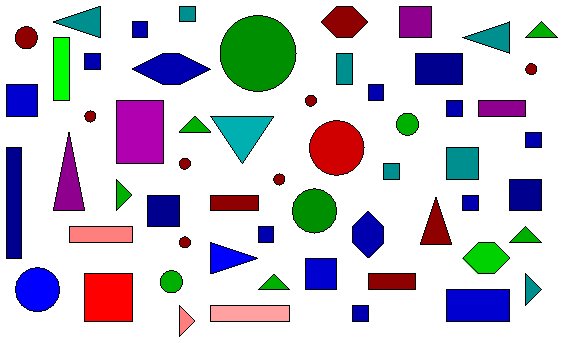
\includegraphics[width=.9\linewidth]{images/objetos2.png}}
        \\ {Imagem original}
    \end{minipage}
    \begin{minipage}{.45\textwidth}
        \centering
        \fbox{
\includegraphics[width=.9\linewidth]{processed/objetos2/border.png}}
        \\ {Bordas da imagem}
    \end{minipage}
    \end{figure}

\section{Extração de Propriedades dos Objetos}
    Para extrair os dados dos objetos, separei eles em componentes conexas e utilizei a biblioteca ``scikit-image''.

    O algoritmo usado para a separação das componentes foi o seguinte:
    \begin{enumerate}
        \item{Para cada pixel da imagem verifique:}
        \begin{itemize}
            \item{Se é objeto.}
            \item{Se não pertence a nenhuma componente no momento.}
        \end{itemize}
        \item{Se ambos são verdade inicie um algoritmo de flood fill a partir desse pixel. (Utilizei BFS)}
    \end{enumerate}

    Na BFS guardei: ID da componente, menor e maior linha atingidas na busca, menor e maior coluna atingidas na busca, coordenadas de todos os pixeis da componente.

    Para gerar as imagens de cada objeto fiz para cada uma das componentes achadas na BFS, um slicing da imagem original de acordo com as linhas e colunas salvas e recolori todos os pixeis desse slicing de acordo com se ele estava ou não na lista de coordenadas salvas daquela componente.

    Tendo essas imagens apenas apliquei a função measure.regionprops da biblioteca citada anteriormente. O resultado detalhado para cada imagem está na pasta processed deste trabalho.

    Para rotular a imagem foi bem simples uma vez que tinha salvo a borda dos objetos na BFS. Utilizei a função cv.putText para escrever a ID da componente que representa aquele objeto e centralizei o texto com o centro do objeto.

    \begin{figure}[H]
    \centering
    \begin{minipage}{.45\textwidth}
        \centering
        \fbox{
\includegraphics[width=.9\linewidth]{images/objetos3.png}}
        \\ {Imagem original}
    \end{minipage}
    \begin{minipage}{.45\textwidth}
        \centering
        \fbox{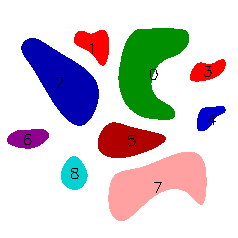
\includegraphics[width=.9\linewidth]{processed/objetos3/regions.png}}
        \\ {Regiões rotuladas}
    \end{minipage}
    \end{figure}

    \begin{center}
    \begin{tabular}{||c c c c c||}
        \hline
        Região & Área & Perímetro & Excentricidade & Solidez \\ [0.5ex] 
        \hline\hline
        0 & 3969 &  313,76 & 0,82 & 0,75 \\ 
        \hline
        1 & 791 & 119,98 & 0,74 & 0,90 \\
        \hline
        2 & 3584 & 259,46 & 0,90 & 0,98 \\
        \hline
        3 & 540 & 99,25 & 0,89 & 0,90 \\
        \hline
        4 & 438 & 88,77 & 0,86 & 0,91 \\ 
        \hline
        5 & 1684 & 174,12 & 0,87 & 0,97 \\ 
        \hline
        6 & 642 & 103,01 & 0,89 & 0,96 \\ 
        \hline
        7 & 3934 & 305,42 & 0,91 & 0,77 \\ 
        \hline
        8 & 675 & 96,33 & 0,62 & 0,97 \\
        \hline
    \end{tabular}
    \\ [1ex] {Propriedades dos objetos}
    \end{center}

\section{Histograma de Área dos Objetos}
    Sem muita complicação, o único detalhe aqui é que a última marcação no eixo x é o máximo entre 4500 e a maior área dos objetos (observe no exemplo 2).

    \subsection{Exemplo 1}
    \begin{figure}[H]
    \centering
    \begin{minipage}{.45\textwidth}
        \centering
        \fbox{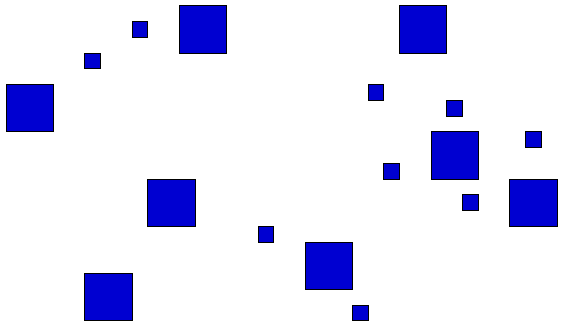
\includegraphics[width=.9\linewidth]{images/objetos1.png}}
        \\ {Imagem original}
    \end{minipage}
    \begin{minipage}{.5\textwidth}
        \centering
        {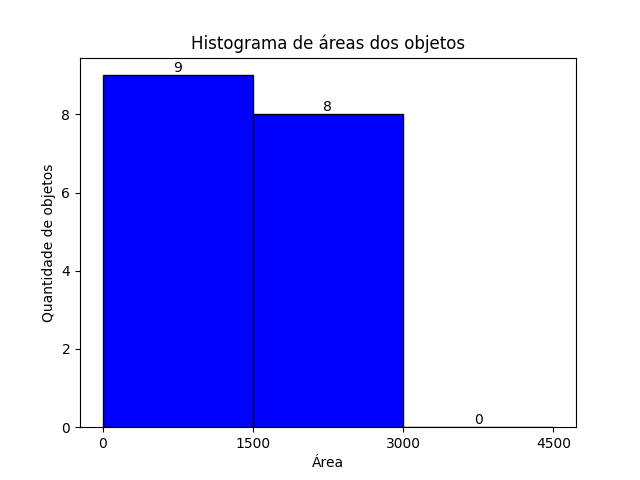
\includegraphics[width=1\linewidth]{processed/objetos1/histogram.png}}
        \\ {Histograma}
    \end{minipage}
    \end{figure}

    \subsection{Exemplo 2}
    \begin{figure}[H]
    \centering
    \begin{minipage}{.45\textwidth}
        \centering
        \fbox{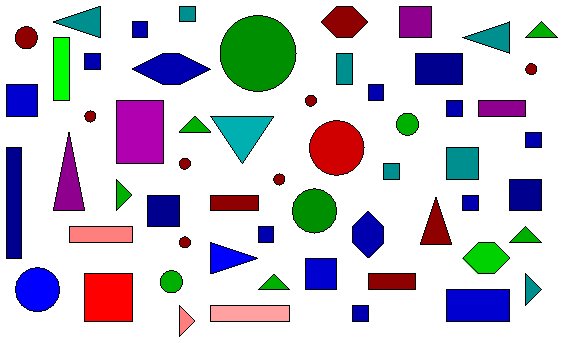
\includegraphics[width=.9\linewidth]{images/objetos2.png}}
        \\ {Imagem original}
    \end{minipage}
    \begin{minipage}{.5\textwidth}
        \centering
        {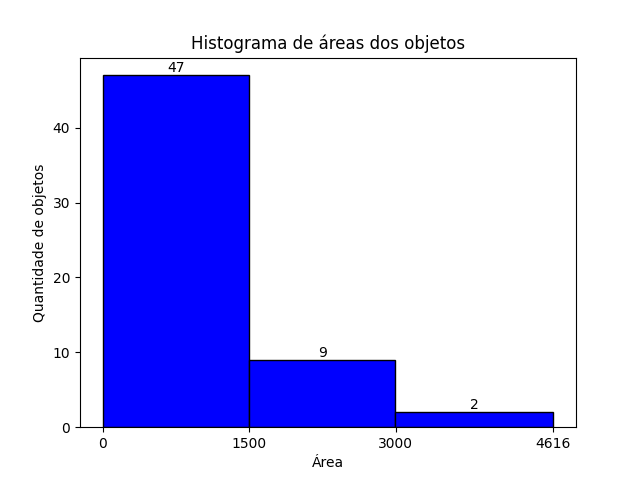
\includegraphics[width=1\linewidth]{processed/objetos2/histogram.png}}
        \\ {Histograma}
    \end{minipage}
    \end{figure}

    \subsection{Exemplo 3}
    \begin{figure}[H]
    \centering
    \begin{minipage}{.45\textwidth}
        \centering
        \fbox{
\includegraphics[width=.6\linewidth]{images/objetos3.png}}
        \\ {Imagem original}
    \end{minipage}
    \begin{minipage}{.5\textwidth}
        \centering
        {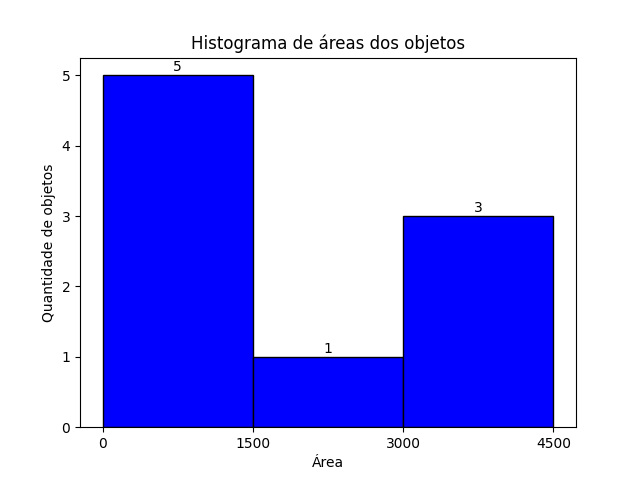
\includegraphics[width=1\linewidth]{processed/objetos3/histogram.png}}
        \\ {Histograma}
    \end{minipage}
    \end{figure}

\section{Bibliografia}
    \href{https://docs.opencv.org/3.1.0/}{Documentação OpenCV}
    
    \href{https://matplotlib.org/stable/index.html}{Documentação Matplotlib}
    
    \href{https://scikit-image.org/docs/stable/index.html}{Documentação Scikit-Image}

\end{document}